\begin{figure}[htp]
	\centering\capstart
	\subfloat[\(\Re\big\{\pixel{\Phi}\big\}\)] % chktex 21
	{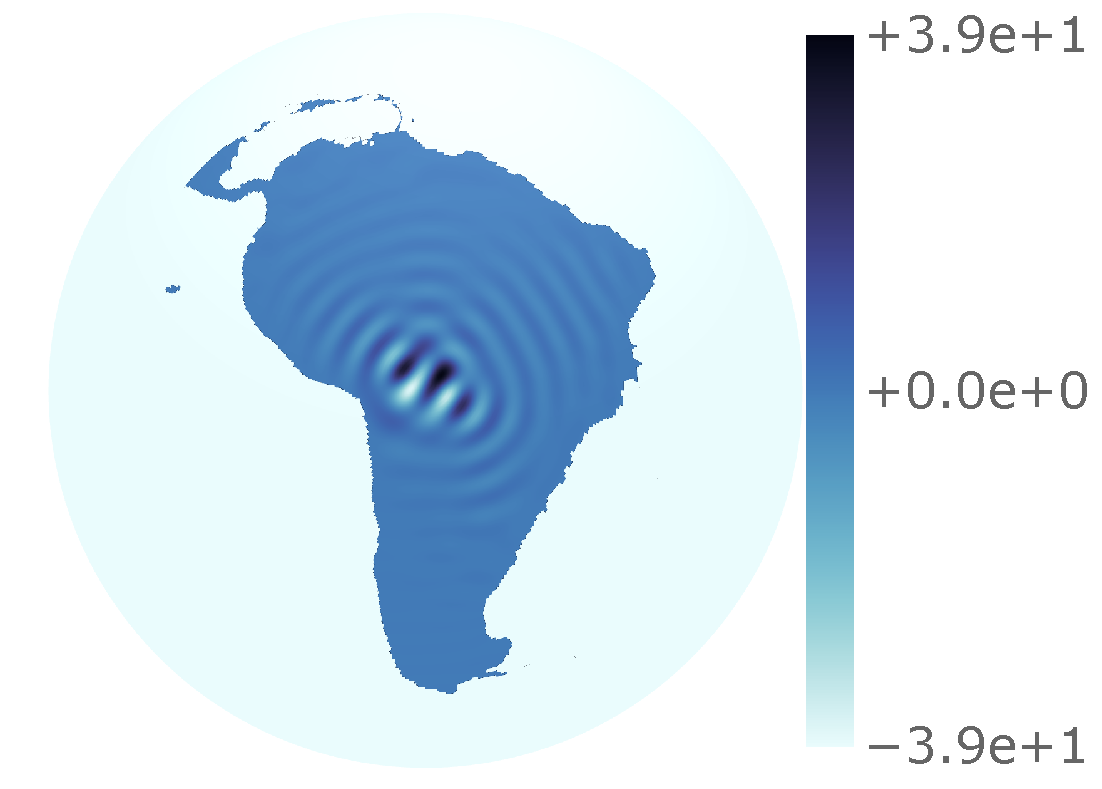
\includegraphics[trim={23 7 3 6},clip,width=.5\textwidth]{slepian_wavelets_south_america_3B_2jmin_scaling_L128_res512_real.pdf}}
	\hfill
	\subfloat[\(\Re\big\{\pixel{\Psi^{2j}}\big\}\)] % chktex 21
	{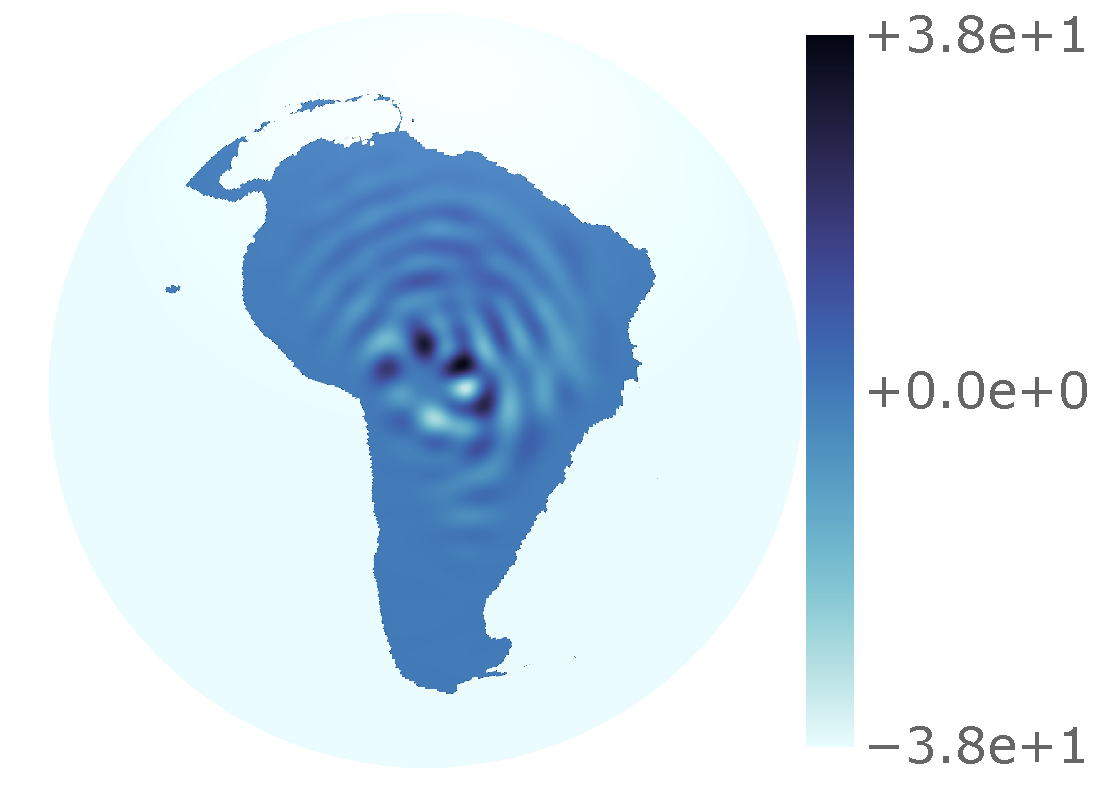
\includegraphics[trim={23 7 3 6},clip,width=.5\textwidth]{slepian_wavelets_south_america_3B_2jmin_2j_L128_res512_real.pdf}}
	\newline
	\subfloat[\(\Re\big\{\pixel{\Psi^{3j}}\big\}\)] % chktex 21
	{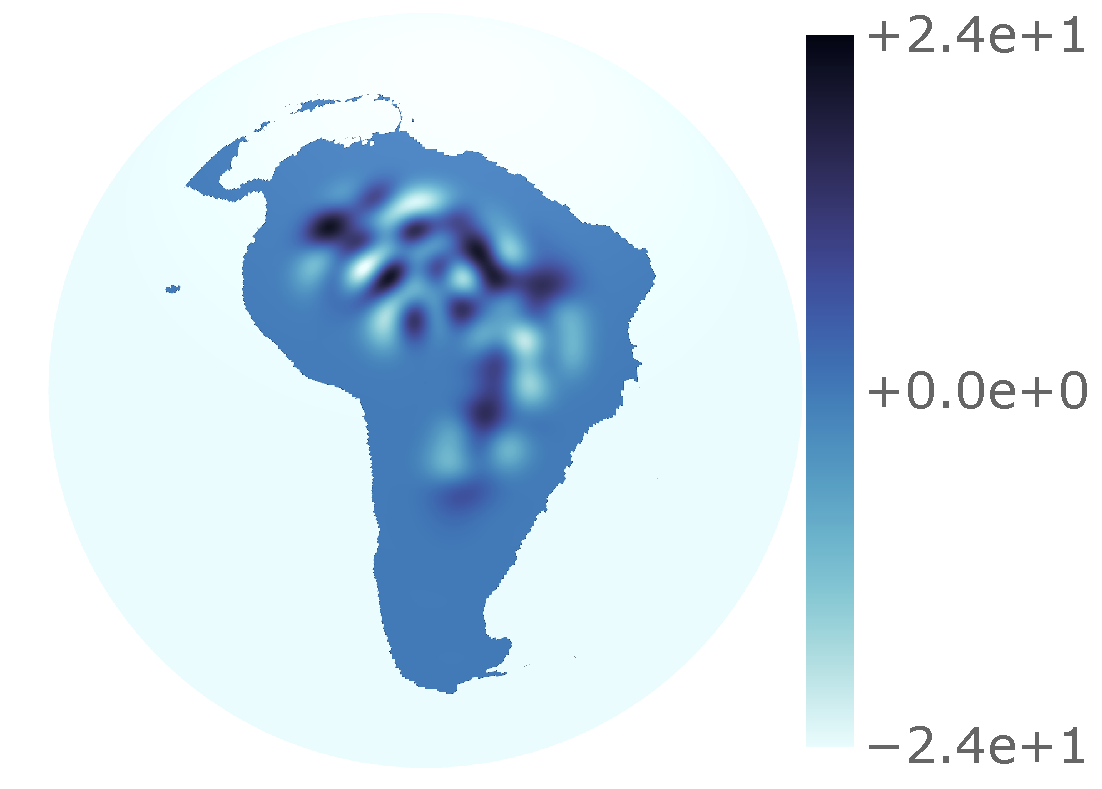
\includegraphics[trim={23 7 3 6},clip,width=.5\textwidth]{slepian_wavelets_south_america_3B_2jmin_3j_L128_res512_real.pdf}}
	\hfill
	\subfloat[\(\Re\big\{\pixel{\Psi^{4j}}\big\}\)] % chktex 21
	{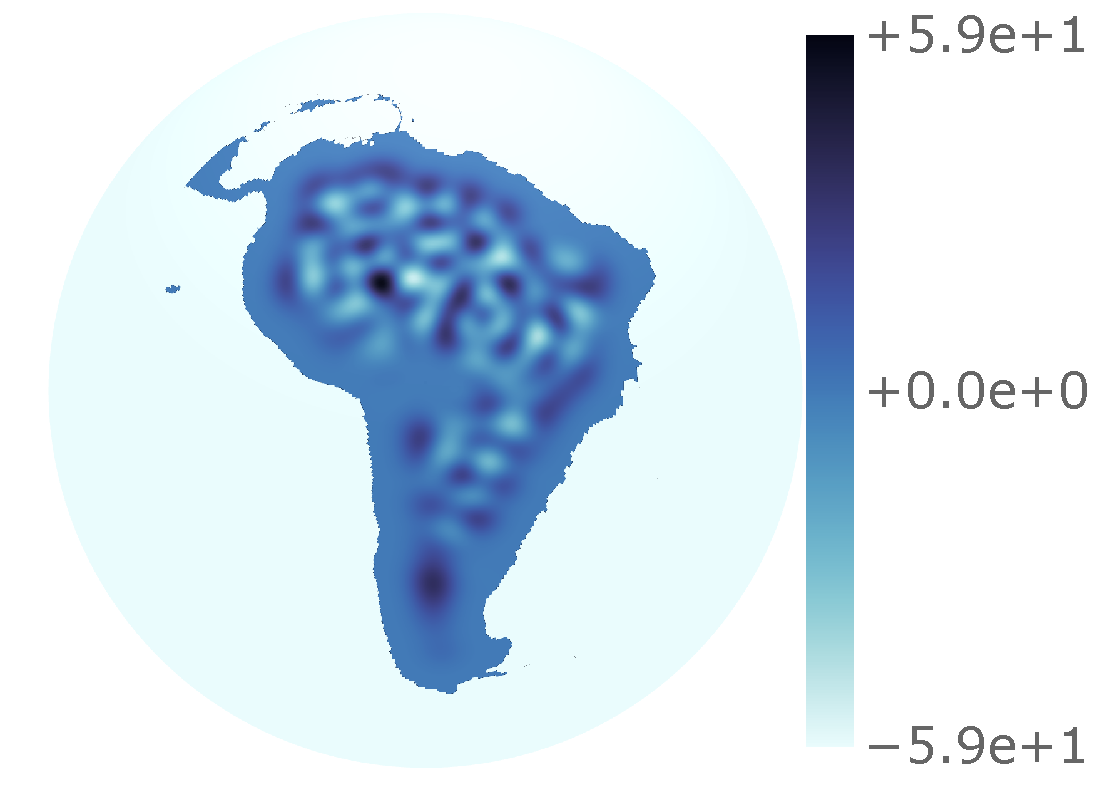
\includegraphics[trim={23 7 3 6},clip,width=.5\textwidth]{slepian_wavelets_south_america_3B_2jmin_4j_L128_res512_real.pdf}}
	\newline
	\subfloat[\(\Re\big\{\pixel{\Psi^{5j}}\big\}\)] % chktex 21
	{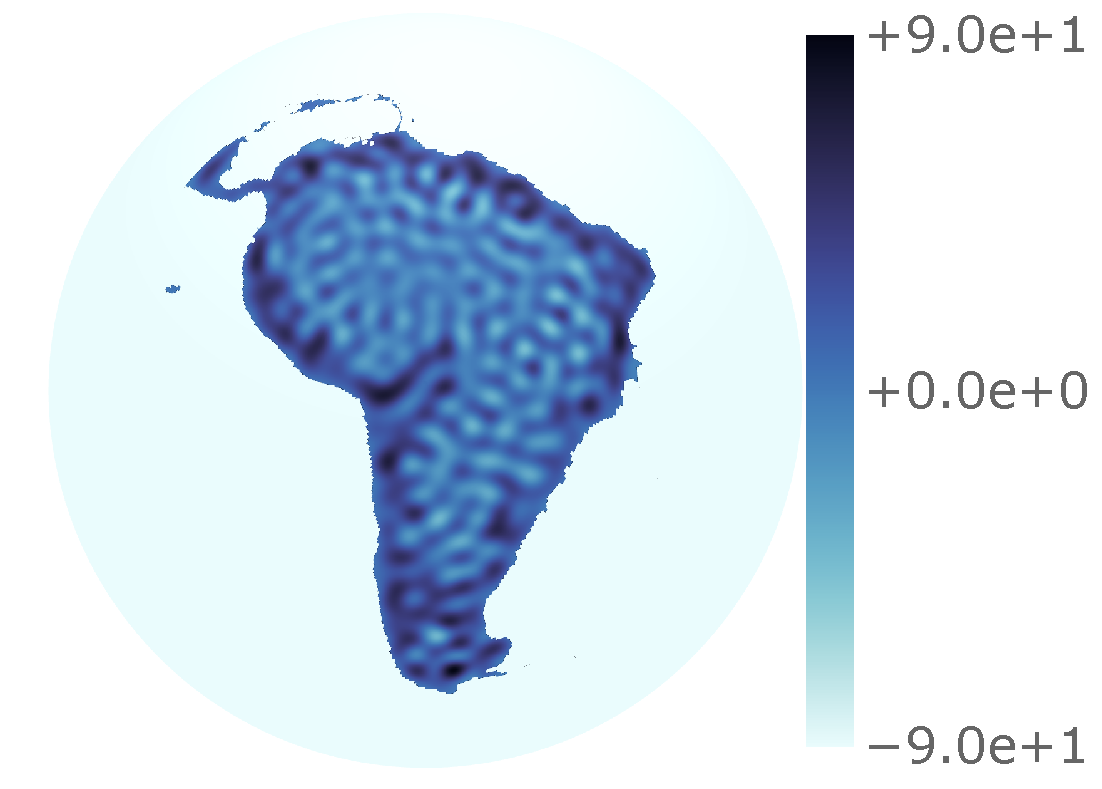
\includegraphics[trim={23 7 3 6},clip,width=.5\textwidth]{slepian_wavelets_south_america_3B_2jmin_5j_L128_res512_real.pdf}}
	\hfill
	\subfloat[\(\Re\big\{\pixel{\Psi^{6j}}\big\}\)] % chktex 21
	{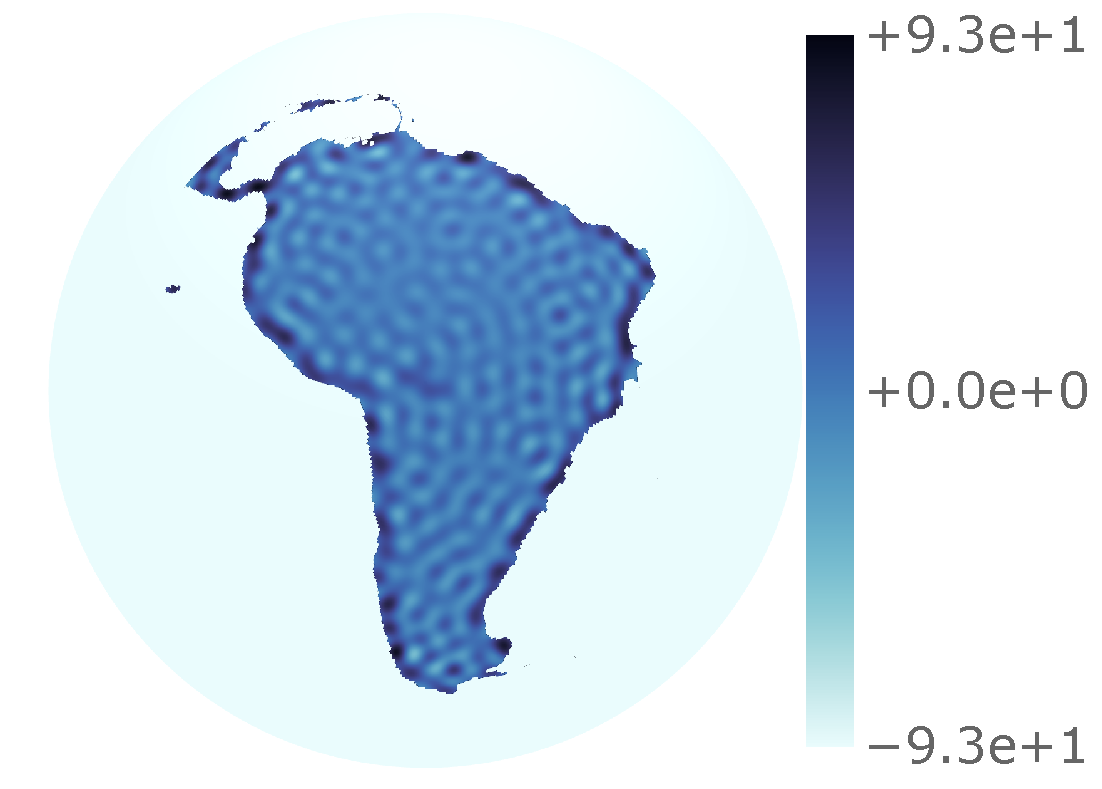
\includegraphics[trim={23 7 3 6},clip,width=.5\textwidth]{slepian_wavelets_south_america_3B_2jmin_6j_L128_res512_real.pdf}}
	\caption[
		The Slepian wavelets of the South America region
	]{
		The scaling function and the wavelets for scales \(j \in \set{2, 3, 4, 5, 6}\) for the South America region shown left-to-right, top-to-bottom.
		The wavelets are constructed through a tiling of the Slepian line using scale-discretised functions, with parameters \(\lambda=3\), \(J_{0}=2\), and bandlimit \(L=128\).
	}\label{fig:chapter3_slepian_wavelets}
\end{figure}
